\documentclass[12pt]{article}
\usepackage[utf8]{inputenc}
\usepackage[russian]{babel}
\usepackage{titlesec}
\usepackage{titling}
\usepackage{graphicx}
\usepackage[russian]{babel}
\usepackage[babel = true]{microtype}
\usepackage[left=10mm,right=10mm, top=15mm,bottom=15mm]{geometry}
\usepackage{amsmath}
\usepackage{mathtools}
\usepackage{array}
\usepackage{wrapfig}
\usepackage{multirow}
\usepackage{tabu}
\let\oldAA\AA
\renewcommand{\AA}{\text{\normalfont\oldAA}}


\setlength{\droptitle}{-5em}

\title{4.1.3. Рефрактометр Аббе}
\date{}

\titleformat{\section}[hang]
{\normalfont\bfseries}
{\thesection.}{0.5em}{}

\titleformat{\subsection}[hang]
{\normalfont\bfseries}
{\thesection.}{0.5em}{}

\begin{document}

\maketitle

\paragraph{Цель работы:}измерить показатели преломления твёрдых и жидких тел в монохроматическом свете.

\paragraph{В работе используются:}технический рефрактометр Аббе; осветитель; набор стеклянных образцов; жидкости с неизвестными показателями преломления (глицерин, этиловый спирт); монохлорнафталин; дистиллированная вода.

\section*{Теоретическая часть:}
\begin{enumerate}
    \item Формула Лоренц—Лорентца, связывающая показатель преломления $n$ изотропного вещества с числом молекул $N$ в единице объёма и поляризуемостью $\alpha$ молекул вещества:
    \begin{equation}\label{eq:1}
        \frac{n^2 - 1}{n^2 + 2} = \frac{4\pi}{3}N\alpha.
    \end{equation}
    Также вводят величину удельной рефракции ($\rho$ --- плотность вещества):
    \[ r = \frac{1}{\rho} \frac{n^2 - 1}{n^2 + 2}. \]
    Тогда:
    \[ r = \frac{4\pi}{3} \frac{\alpha}{m_0} = \mathrm{const} \]
    
    \item Для смеси веществ хорошо выполняется соотношение:
    \[ r = c_1 r_1 + c_2 r_2 + \dots, \]
    где $r_1, r_2, \dots $ --- удельные рефракции компонетов, а $ c_1, c_2,\dots $ --- их массовые доли. То есть, рефракция обладает свойством аддитивности. \\
    Также вводят понятие атомной рефракции:
    \[ R = A r,\]
    где $A$ --- атомная масса элемента. И, аналогично, вводят молекулярную рефракцию $R_M$:
    \[ R_M = M r = \frac{M}{\rho} \frac{n^2 - 1}{n^2 + 2} = \frac{4\pi}{3}N_A \alpha. \]
    Тогда:
    \[ R_M = q_1 A_1 r_1 + q_2 A_2 r_2 + \dots = q_1 R_1 + q_2 R_2 + \dots \]
    Определив в ходе работы рефрацкции воды, глицерина и этилового спирта, получим систему:
    \begin{align*}
        &R_{H_2 O} = 2R_H +R_O                   \\
        &R_{C_3 H_8 O_3} = 3R_C + 8R_H + 3R_O    \\
        &R_{C_2 H_6 O} = 2R_C + 6R_H + R_O
    \end{align*}
\end{enumerate}
\newpage
    
\section*{Экспериментальная установка:}
Принцип работы рефрактометра Аббе
    \[ \sin{\varphi_{\text{пр}}} = \frac{n_1}{n_2} \]
    
    \begin{figure}[h!]
        \noindent\centering{
            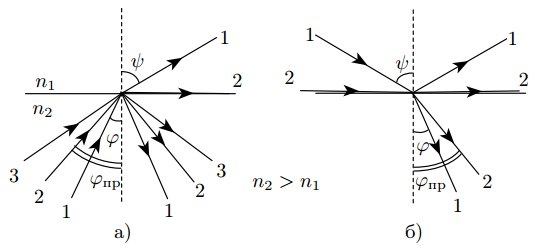
\includegraphics[height = 6cm]{Selection_045.png}
        }
        \caption{Предельный угол полного внутреннего отражения (а) и предельный угол преломления (б)}
    \end{figure}   
    
    Для измерения показателей преломления используются 2 метода – метод полного внутреннего отражения и метод скользящего луча.
    
    \begin{figure}[h!]
        \noindent\centering{
            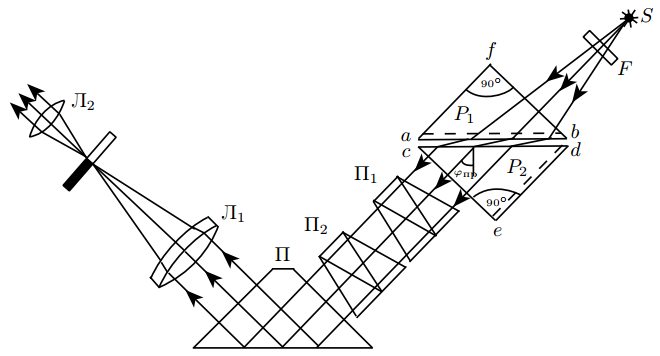
\includegraphics[height = 8cm]{Selection_046.png}
        }
        \caption{Ход лучей в рефрактометре при измерении показателя преломления жидкости методом скользящего луча}
    \end{figure} 
    
    \begin{figure}[h!]
        \noindent\centering{
            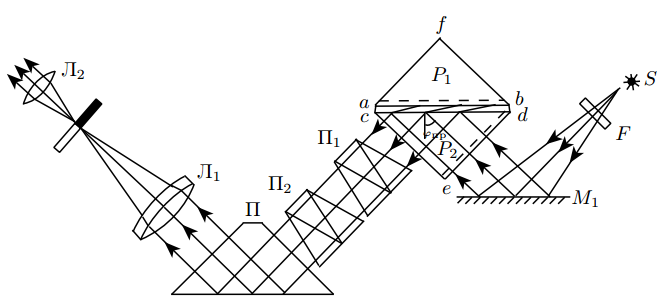
\includegraphics[height = 8cm]{Selection_047.png}
        }
        \caption{Ход лучей в рефрактометре при измерении показателя преломления жидкости методом полного внутреннего отражения}
    \end{figure} 
\newpage

\section*{Ход работы:}
\begin{enumerate}
    \item Измерим показатели преломления 3 стеклянных образцов используя оба метода. Для каждого образца проведем по 5 измерений каждым методом. Сведем результаты в таблицу:
    
    \begin{table}[h!]
        \centering
        \begin{tabular}{| c | c | c | c | c | c | c | c |} 
            \hline
            Номер эксперимента & 1 & 2 & 3 & 4 & 5 & $\bar{n}$ & $\sigma_n$ \\
            \hline
            $n_1$ & 1.5135 & 1.514 & 1.514 & 1.513 & 1.512 & 1.5133 & $6 \cdot 10^{-4}$ \\
            \hline
            $n_2$ & 1.6535 & 1.653 & 1.654 & 1.652 & 1.655 & 1.6535 & $7 \cdot 10^{-4}$ \\
            \hline
            $n_3$ & 1.652 & 1.6515 & 1.652 & 1.650 & 1.653 & 1.6517 & $7 \cdot 10^{-4}$ \\
            \hline
        \end{tabular}
        \caption{Метод скользящего луча}
    \end{table}   
    
    \begin{table}[h!]
        \centering
        \begin{tabular}{| c | c | c | c | c | c | c | c |} 
            \hline
            Номер эксперимента & 1 & 2 & 3 & 4 & 5 & $\bar{n}$ & $\sigma_n$ \\
            \hline
            $n_1$ & 1.513 & 1.5145 & 1.5135 & 1.514 & 1.525 & 1.516 & $6 \cdot 10^{-4}$ \\
            \hline
            $n_2$ & 1.6485 & 1.6495 & 1.650 & 1.649 & 1.653 & 1.650 & $7 \cdot 10^{-4}$ \\
            \hline
            $n_3$ & 1.6525 & 1.657 & 1.658 & 1.66 & 1.65 & 1.6555 & $7 \cdot 10^{-4}$ \\
            \hline
        \end{tabular}
        \caption{Метод полного внутреннего отражения}
    \end{table} 
    
    Описание образцов:
    \begin{enumerate}
        \item толстый восьмиугльник
        \item тонкий маленькй прямоугольник
        \item тонкий большой прямоугольник
    \end{enumerate}

    \item Аналогично измерим показатели преломления глицерина и этилового спирта.
    
    \begin{table}[h!]
        \centering
        \begin{tabular}{| c | c | c | c | c | c | c | c |} 
            \hline
            Номер эксперимента & 1 & 2 & 3 & 4 & 5 & $\bar{n}$ & $\sigma_n$ \\
            \hline
            $n_{C_3 H_8 O_3}$ & 1.451 & 1.452 & 1.4505 & 1.4515 & 1.45 & 1.451 & $2 \cdot 10^{-4}$ \\ 
            \hline
            $n_{C_2 H_6 O}$ & 1.395 & 1.361 & 1.360 & 1.3605 & 1.359 & 1.36 & $5 \cdot 10^{-4}$ \\
            \hline
        \end{tabular}
        \caption{Метод скользящего луча}
    \end{table}   
    
    \begin{table}[h!]
        \centering
        \begin{tabular}{| c | c | c | c | c | c | c | c |} 
            \hline
            Номер эксперимента & 1 & 2 & 3 & 4 & 5 & $\bar{n}$ & $\sigma_n$ \\
            \hline
            $n_{C_3 H_8 O_3}$ & 1.4505 & 1.4515 & 1.45 & 1.452 & 1.451 &  1.451 & $4 \cdot 10^{-4}$ \\ 
            \hline
            $n_{C_2 H_6 O}$ & 1.390 & 1.360 & 1.3605 &  1.361  & 1.3595 & 1.36 & $6 \cdot 10^{-4}$ \\
            \hline
        \end{tabular}        
        \caption{Метод полного внутреннего отражения}
    \end{table}
    \newpage
    Итого имеем:
    \[ n_{C_3 H_8 O_3} = 1.451 \pm 0.0001, \ n_{C_2 H_6 O} = 1.36 \pm 0.0005. \]
    \item Теперь можем вычислить молекулярные рефракции и поляризуемости по формуле \eqref{eq:1} :
    \begin{align*}
        &R_{H_2 O} = 3.67 \frac{\text{см}^3}{\text{моль}} \\
        &R_{C_3 H_8 O_3} = 20.35 \frac{\text{см}^3}{\text{моль}} \\
        &R_{C_2 H_6 O} = 12.86 \frac{\text{см}^3}{\text{моль}}
    \end{align*}
    \item Решая сиситему линейных уравнений, находим атомарные рефракции углерода, водорода и кислорода: 
     \begin{align*}
        &R_{H} = 1.11 \frac{\text{см}^3}{\text{моль}} \\
        &R_{O} = 1.45 \frac{\text{см}^3}{\text{моль}} \\
        &R_{C} = 2.37 \frac{\text{см}^3}{\text{моль}}
    \end{align*}
    \item Предполагая справедливым правило аддитивности, можем вычислить рефракцию для этилового спирта и его показатель преломления:
    \[ R_{C H_4 O} = 8.27 \frac{\text{см}^3}{\text{моль}}, \ n_{C H_4 O}  = 1.33 \]
    Табличное значение: $n = 1.33$, из чего можно сделать вывод, что наши эккспериментальные данные хорошо согласовываются с теорией. \\
    Для льда по нашим данным получаем: $n_{\text{лёд}} = 1.294$, при табличном значении $n = 1.31$
\end{enumerate}

\section*{Вывод:} 
Измерили показатели преломления твердых и жидких тел в монохроматическом свете при помощи рефрактометра Аббе. Используя метод полного внутреннего отражения и метод скользящего луча, получили одинаковые результаты с большой точностью. Убедились в аддитивности рефракции.
\end{document}
